%%
%% This is file `sample-sigconf.tex',
%% generated with the docstrip utility.
%%
%% The original source files were:
%%
%% samples.dtx  (with options: `sigconf')
%% 
%% IMPORTANT NOTICE:
%% 
%% For the copyright see the source file.
%% 
%% Any modified versions of this file must be renamed
%% with new filenames distinct from sample-sigconf.tex.
%% 
%% For distribution of the original source see the terms
%% for copying and modification in the file samples.dtx.
%% 
%% This generated file may be distributed as long as the
%% original source files, as listed above, are part of the
%% same distribution. (The sources need not necessarily be
%% in the same archive or directory.)
%%
%%
%% Commands for TeXCount
%TC:macro \cite [option:text,text]
%TC:macro \citep [option:text,text]
%TC:macro \citet [option:text,text]
%TC:envir table 0 1
%TC:envir table* 0 1
%TC:envir tabular [ignore] word
%TC:envir displaymath 0 word
%TC:envir math 0 word
%TC:envir comment 0 0
%%
%%
%% The first command in your LaTeX source must be the \documentclass
%% command.
%%
%% For submission and review of your manuscript please change the
%% command to \documentclass[manuscript, screen, review]{acmart}.
%%
%% When submitting camera ready or to TAPS, please change the command
%% to \documentclass[sigconf]{acmart} or whichever template is required
%% for your publication.
%%
%%
\documentclass[sigconf]{acmart}

\usepackage[T1]{fontenc}

\usepackage[latin9]{inputenc}
% \usepackage[a4paper]{geometry}
% \geometry{verbose,tmargin=1in,bmargin=1in,lmargin=1in,rmargin=1in}
% \usepackage{babel}
\usepackage{amsmath}
\usepackage{amsthm}
% \usepackage{amssymb}
\usepackage{stmaryrd}

\usepackage{soul}
\usepackage{xspace}
\usepackage{csquotes}
\usepackage{booktabs}
\usepackage{multirow}

\usepackage{thmtools}
\usepackage{thm-restate}

\usepackage{backnaur}
\usepackage{stmaryrd}
\usepackage{oplotsymbl}
\usepackage{enumerate}
\usepackage{algorithm}
\usepackage{algorithmicx}
\usepackage{algpseudocode}
\usepackage{xspace}
\usepackage{tcolorbox}


\algnotext{EndFor}
\algnotext{EndIf}
\algnotext{EndWhile}


\usepackage{hyperref}
\usepackage{color}

%% for plots
\usepackage{tikz}
\usetikzlibrary{calc}
\usepackage{pgfplots}
\usepackage{pgfplotstable}
\usepackage{subcaption}
\usepackage[font=small,labelfont=bf,tableposition=top]{caption}



\tikzset{
	POINTS/.style={solid, mark=square*, red},
	V1COALESCED/.style={solid, mark=square, blue},
	V2COALESCED/.style={solid, mark=o, green},
}

\newcommand{\legpoints}{\ensuremath{\tuples}\xspace}
\newcommand{\legvi}{\ensuremath{\tuplest}\xspace}
\newcommand{\legvii}{\ensuremath{\tuplesd}\xspace}

\pgfplotsset{
	every axis/.append style={
		legend columns=-1,
		legend style={
			at={(0.5,1)},
			anchor=south,
			font=\tiny,
			draw=none,
			fill=none,
			row sep=0.01cm
		},
		height = 3.5cm,
		width = 4.3cm,
		xlabel near ticks,
		ylabel near ticks,
		legend cell align = left,
		label style = {font=\scriptsize},
	},
	every tick label/.append style={
		font=\tiny
	},
}
%% end for plots




%%
%% \BibTeX command to typeset BibTeX logo in the docs
% \AtBeginDocument{%
%   \providecommand\BibTeX{{%
%     Bib\TeX}}}

%% Rights management information.  This information is sent to you
%% when you complete the rights form.  These commands have SAMPLE
%% values in them; it is your responsibility as an author to replace
%% the commands and values with those provided to you when you
%% complete the rights form.
% \setcopyright{acmcopyright}
% \copyrightyear{2018}
% \acmYear{2018}
% \acmDOI{XXXXXXX.XXXXXXX}

%% These commands are for a PROCEEDINGS abstract or paper.
% \acmConference[Conference acronym 'XX]{Make sure to enter the correct
  % conference title from your rights confirmation emai}{June 03--05,
  % 2018}{Woodstock, NY}
%%
%%  Uncomment \acmBooktitle if the title of the proceedings is different
%%  from ``Proceedings of ...''!
%%
%%\acmBooktitle{Woodstock '18: ACM Symposium on Neural Gaze Detection,
%%  June 03--05, 2018, Woodstock, NY}
% \acmPrice{15.00}
% \acmISBN{978-1-4503-XXXX-X/18/06}


%%
%% Submission ID.
%% Use this when submitting an article to a sponsored event. You'll
%% receive a unique submission ID from the organizers
%% of the event, and this ID should be used as the parameter to this command.
%%\acmSubmissionID{123-A56-BU3}

%%
%% For managing citations, it is recommended to use bibliography
%% files in BibTeX format.
%%
%% You can then either use BibTeX with the ACM-Reference-Format style,
%% or BibLaTeX with the acmnumeric or acmauthoryear sytles, that include
%% support for advanced citation of software artefact from the
%% biblatex-software package, also separately available on CTAN.
%%
%% Look at the sample-*-biblatex.tex files for templates showcasing
%% the biblatex styles.
%%

%%
%% The majority of ACM publications use numbered citations and
%% references.  The command \citestyle{authoryear} switches to the
%% "author year" style.
%%
%% If you are preparing content for an event
%% sponsored by ACM SIGGRAPH, you must use the "author year" style of
%% citations and references.
%% Uncommenting
%% the next command will enable that style.
%%\citestyle{acmauthoryear}


\input{../macros/colors}
\input{../macros/comments}
\input{../macros/macros_j}
\input{../macros/macros_a}
\input{../defines_sql}

%%
%% end of the preamble, start of the body of the document source.
\begin{document}

%%
%% The "title" command has an optional parameter,
%% allowing the author to define a "short title" to be used in page headers.
\title{Compact Answers to Temporal Regular Path Queries (Supplementary Material)}

%%
%% The "author" command and its associated commands are used to define
%% the authors and their affiliations.
%% Of note is the shared affiliation of the first two authors, and the
%% "authornote" and "authornotemark" commands
%% used to denote shared contribution to the research.

%%
%% By default, the full list of authors will be used in the page
%% headers. Often, this list is too long, and will overlap
%% other information printed in the page headers. This command allows
%% the author to define a more concise list
%% of authors' names for this purpose.
% \renewcommand{\shortauthors}{Trovato et al.}

%%
%% The abstract is a short summary of the work to be presented in the
%% article.
% \begin{abstract}
    % \input{input/abstract.tex}
% \end{abstract}

%%
%% The code below is generated by the tool at http://dl.acm.org/ccs.cfm.
%% Please copy and paste the code instead of the example below.
%%
% \begin{CCSXML}
% <ccs2012>
%  <concept>
%   <concept_id>10010520.10010553.10010562</concept_id>
%   <concept_desc>Computer systems organization~Embedded systems</concept_desc>
%   <concept_significance>500</concept_significance>
%  </concept>
%  <concept>
%   <concept_id>10010520.10010575.10010755</concept_id>
%   <concept_desc>Computer systems organization~Redundancy</concept_desc>
%   <concept_significance>300</concept_significance>
%  </concept>
%  <concept>
%   <concept_id>10010520.10010553.10010554</concept_id>
%   <concept_desc>Computer systems organization~Robotics</concept_desc>
%   <concept_significance>100</concept_significance>
%  </concept>
%  <concept>
%   <concept_id>10003033.10003083.10003095</concept_id>
%   <concept_desc>Networks~Network reliability</concept_desc>
%   <concept_significance>100</concept_significance>
%  </concept>
% </ccs2012>
% \end{CCSXML}

% \ccsdesc[500]{Computer systems organization~Embedded systems}
% \ccsdesc[300]{Computer systems organization~Redundancy}
% \ccsdesc{Computer systems organization~Robotics}
% \ccsdesc[100]{Networks~Network reliability}

%%
%% Keywords. The author(s) should pick words that accurately describe
%% the work being presented. Separate the keywords with commas.
% \keywords{graph databases, temporal graphs, regular path queries}
%% A "teaser" image appears between the author and affiliation
%% information and the body of the document, and typically spans the
%% page.
% \begin{teaserfigure}
%   \includegraphics[width=\textwidth]{input/figures/sampleteaser}
%   \caption{Seattle Mariners at Spring Training, 2010.}
%   \Description{Enjoying the baseball game from the third-base
%   seats. Ichiro Suzuki preparing to bat.}
%   \label{fig:teaser}
% \end{teaserfigure}


% \begin{teaserfigure}
%     \input{input/figures/table.tex}
% \end{teaserfigure}
% \received{20 February 2007}
% \received[revised]{12 March 2009}
% \received[accepted]{5 June 2009}

%%
%% This command processes the author and affiliation and title
%% information and builds the first part of the formatted document.
\maketitle

\onecolumn


 
\section{Inductive representation}
\label{sec:inductive}


\subsection{$\evalcitdbe{q}$}

\subsubsection{Definition}
\label{sec:evalbe_def}

\subsubsection{Correctness}
\label{sec:evalbe_correct}

\para{$\path_1/\path_2$}
Let $\u_1 = \tup{o_1, o_2, \tau_1, \delta_1}$ and $\u_2 = \tup{o_3, o_4, \tau_2, \delta_2}$,
with $o_2 = o_3$.

And let  $\u_1 \tjoin \u_2 = \tup{o_1, o_4, \tau'_1, \delta_1 + \delta_2, b,e}$,
with
\begin{align*}
\tau'_1 &=  (((\tau_1 + \delta_1) \cap \tau_2) \ominus \delta_1) \cap \tau_1\\
  b &= \max(b_1, b_2 - b_{\delta_1})\\
  e &= \min(e_1, e_2 - e_{\delta_1})
\end{align*}



For each $i \in \{1,2\}$ and $t \in \tau_i$,
we use $\delta_i(t)$ for the interval
\[\ld{\delta_{i}}\ b_{\delta_i} + \max(0, b_i - t) \ ,\ e_{\delta_i} - \max(0, t - e_i)\ \rd{\delta_{i}}\]
And similarly to what we did for $\tuplestd$,
we use $R_i$ for be the binary relation over $\td$ specified by the time points and distances in $\u_i$,
i.e.~$R_i = \{(t,t + d) \mid t \in \tau_i, d \in \delta_i(t)\}$.

Then the intervals in the set $\u_1 \tjoin \u_2$ should intuitively represent this relation $R_1 \join R_2$, i.e.

with
\begin{align*}
\tau'_1 &=  (((\tau_1 + \delta_1) \cap \tau_2) \ominus \delta_1) \cap \tau_1\\
  b &= \max(b_1, b_2 - b_{\delta_1})\\
  e &= \min(e_1, e_2 - e_{\delta_1})
%   \begin{cases}
%     b_1 &\te{if} b_2 \le b_1 + b_{\delta_1}\\
%     b_2 - b_{\delta_1} &\te{otherwise}
%   \end{cases}
% &
 % e =
 %  \begin{cases}
 %    e_1 &\te{if} e_1 + e_{\delta_1} \le e_2 \\
 %    e_2 - e_{\delta_1} &\te{otherwise}
 %  \end{cases}
\end{align*}


The proof that 

Now let $t \in $



%%% Local Variables:
%%% mode: latex
%%% TeX-master: "../appendix"
%%% End:

 
\section{Finiteness}
\label{sec:finite}


%%% Local Variables:
%%% mode: latex
%%% TeX-master: "../appendix"
%%% End:

 
\section{Complexity of query answering}
\label{sec:complexity}


%%% Local Variables:
%%% mode: latex
%%% TeX-master: "../appendix"
%%% End:

 
\section{Minimization}
\label{sec:minimization}


%%% Local Variables:
%%% mode: latex
%%% TeX-master: "../appendix"
%%% End:

 
\section{Size of compact answers}
\label{sec:size}


%%% Local Variables:
%%% mode: latex
%%% TeX-master: "../appendix"
%%% End:

 % \section{Complexity of \pbm}
\label{sec:proofs_complexity}


        % \noindent Let $I_b = \{ b \in \rat \mid b = b_{\alpha} \text{ or } b = e_{\alpha}
        % \text{ for every }
    % \alpha \text{ specified in } compac(G) \text{ or  } \alpha \text{ specified in } q \} $

    % Let $\alpha_{1},\dotsc,\alpha_{k}$ be a finite set of intervals, where $\alpha_i$ is either specified in the
    % graph or in the query.



% \propPspaceMemb*
\begin{proof}
    $ $\newline

    \noindent Let $I_{\Omega}$ be the set of rational numbers $\mathrm{b}$ such that $\mathrm{b} = b_{\tau}$ or $b =
    e_{\tau}$ for every interval
    $\tau$ specified in both $compac(G)$ and in $q$. Since $b \in \rat$, so it can be
    specified as a fraction, i.e., $\frac{p}{q}$, where $p,q \in
    \mathbb{Z}$ and $q \neq 0$. We say that
    $\mathrm{denom}(\frac{p}{q})=q$. Then $g$ be the
    granularity of the graph,
    i.e.,
    % \[
    %     g=\prod_{i=1}^k \mathrm{denom}(b_{\alpha_i}) \times \mathrm{denom}(e_{\alpha_i})
    % \]
    \[
        g=\prod_{i=1}^{\lvert I_{\Omega} \rvert} \mathrm{denom}(\mathrm{b})
    \]

    \begin{lemma}\label{lemma:interval_boundaries}
    If $\langle o_1,o_2,\tau,d \rangle$ is a compact answer to $q$, then the denominator of $b_{\tau}$ and
    and the denominator of $e_{\tau}$ divide $g$.

  \end{lemma}
  \begin{proof}

      \emph{Proof sketch}. We know that we navigate temporal dimension of $G$ using only $\tndelta$
      operator. The definition of $\evalcit{\tndelta}$ requires exactly two
      arithmetic operations addition and subtraction. If the denominators of starting interval
      divide $g$, then after applying $\tndelta$, the denominators of ending
      interval also divide $g$.    

  \end{proof}


    % That means that the denominator of each interval boundary specified in the graph and in the query divides $g$.

    
    \noindent Let $K=\{\frac{j}{2g} \mid j \in \mathbb{Z} \}$. Let $l$ be the
    greatest lower bound in $K$ such that $l < b_{\tau}$ and $l = b_{\tau} -
    \frac{1}{2g}$. Similarly, let $m$ be the lowest upper bound in $K$ such that $m >
    e_{\tau}$ and $m = e_{\tau} + \frac{1}{2g}$. \\
    
    \noindent We claim that $\langle o_1,o_2,\tau,d \rangle \in \evalcit{q}$
    iff $\langle
    o_1, l,o_2,l+d \rangle \not\in
    \eval{q}$ and $\langle
    o_1,m,o_2,m+d \rangle \not\in
    \eval{q}$ and for every $k \in K$, if $k \in \tau$, then $\langle o_1, k, o_2, k+d \rangle \in \eval{q}$. \\

    \noindent $(\implies).$ Trivially holds from the definition of $\evalcit{q}$. \\\\
    \noindent $(\impliedby).$ If $\langle
    o_1, l,o_2,l+d \rangle \not\in
    \eval{q}$ and $\langle
    o_1,m,o_2,m+d \rangle \not\in
    \eval{q}$ and for every $k \in K$, if $k \in \tau$, then $\langle o_1, k,
    o_2, k+d \rangle \in \eval{q}$. Then $\langle o_1,o_2,\tau,d \rangle \in
    \evalcit{q}$. \\

    \noindent We prove the above statement by contradiction. 

    % We  assume
    % $\langle
    % o_1, l,o_2,l+d \rangle \not\in
    % \eval{q}$ and $\langle
    % o_1,m,o_2,m+d \rangle \not\in
    % \eval{q}$ and for every $k \in K$, if $k \in \alpha$, then $\langle o_1, k,
    % o_2, k+d \rangle \in \eval{q}$ is true and 


    We assume for every $k \in K$, if $k \in \tau$, then $\langle o_1, k,
    o_2, k+d \rangle \in \eval{q}$. Assume $\langle o_1,o_2,\tau,d
    \rangle \in \evalcit{q}$ is false. For the simplicity, assume $q$ is a
    boolean query. Then $q$ does not continuously
    hold on $\tau$ which implies there is a $t \in \tau$ such that $t \not\in K$ and $q$ does not hold on $t$.
    % $\langle o_1, t,
    % o_2, t+d \rangle \not\in \eval{q}$.
Let $p$ be the predecessor of $t$ and $s$ be the successor of t. Since $p,s
    \in K$, so by our assumption $q$ holds on $p$ and $s$.  
    % $\implies$ $\langle o_1, p,
    % o_2, p+d \rangle \in \eval{q}$ and $\langle o_1, s,
    % o_2, s+d \rangle \in \eval{q}$ from the assumption. \\\\
Then $p$ and $s$ are the boundaries of the intervals where $q$ holds. From the
definition of $K$, the numerator of every $k \in K$ is either even or odd and if the numerator of $k$ 
is odd then, $\mathrm{denom}(k)$ is $2g$. Since $t$ lies
between $p$ and $s$ and $p,s \in K$, so either the numerator of $p$ is odd or
the numerator of $s$ is odd. As shown in Figure. \ref{fig:pspace}, the numerator of $p$
is odd. Since we know that if the numerator of $k \in K$ is odd, then the denominator is $2g$ which does
not divide
$g$, which implies either $p$ does not divide $g$ or $s$ does not divide $g$
but according to our lemma \ref{lemma:interval_boundaries} both $p$ and $s$ must divide $g$ that means either $q$ does not hold on $p$ or $q$ does not hold on $s$ that contradicts with our assumption that $q$ holds on both $p$ and $s$.\\ 


\end{proof}


\begin{figure}[!htbp]
\centering
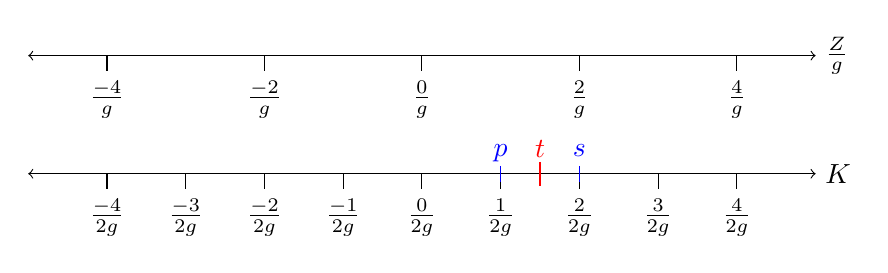
\begin{tikzpicture}

   \draw[<->] (-5,0) -- (5,0) node[right] {$K$};
  \foreach \x in {-4,...,4}
    \draw (\x, 0) -- (\x, -0.2) node[below]{\bfseries
        $\frac{\x}{2g}$};
    % \draw[fill] (1.5,0) circle (0.10) node [yshift=0.6cm, anchor=north]
    %     {$\alpha_2$};
    \draw[red, thick] (1.5,0.15) -- (1.5,-0.15) node [yshift=0.7cm, anchor=north]
        {$t$};
    \draw[blue] (1,0.1) -- (1,-0.1) node [yshift=0.6cm, anchor=north]
        {$p$};
    \draw[blue] (2,0.1) -- (2,-0.1) node [yshift=0.6cm, anchor=north]
        {$s$};

    % first number line
    \draw[<->, yshift=1.5cm] (-5,0) -- (5,0) node[right] {$\frac{\mathbb{Z}}{g}$};
  \foreach \x in {-4,-2,...,4}
    \draw[yshift=1.5cm] (\x, 0) -- (\x, -0.2) node[below]{\bfseries
        $\frac{\x}{g}$};

\end{tikzpicture}
\caption{caption}
\label{fig:pspace}
\end{figure}

\adnanbox{TODO: the case "$\langle o_1,o_2,\alpha,d \rangle$ is maximum" is still pending.} 



% \propPspaceHard*

\begin{proof}
    $ $\newline
    We will reduce the problem of deciding whether a given pairs of temporal
    objects $\langle o_1,o_2,t_1,t_2 \rangle$, a trpq $q$, and a temporal
    property graph $G$, is $\langle o_1,o_2,t_1,t_2  \rangle$ an answer to
    $q$ over $G$ to the problem of deciding whether $\langle o_1,o_2,\alpha,d
    \rangle$ is a \emph{compact} answer to query $q$ over the compact representation of $G$. \\

    \begin{itemize}
        \item check if $\xi(o_1,t_1) = false$ or
            $\xi(o_2, t_2) = false$, then $\langle
            o_1,o_2,t_1,t_2 \rangle$ is not an answer to $q$.
        \item otherwise, we will construct a new graph $G'$ as follows:
            \begin{itemize}
              % \item add two fresh nodes $n_1$ and $n_2$ to the graph $G$, each with
            % time interval $\Omega$
        \item add two fresh properties: $p_1$ on $o_1$ with value $v_1$ at
            interval $[t_1)$, and $p_2$ on $o_2$ with the value $v_2$ at
            the interval $[t_2)$, respectively

            \end{itemize}
        \end{itemize}
        Now consider the query
        \[
            q' = p_1 \mapsto v_1/q/p_2 \mapsto v_2
        \]

\noindent Note that the construction of $G'$ and $q'$ can be done in \emph{polynomial} time. \\

\noindent We claim that $\langle o_1,o_2,t_1,t_2 \rangle$ is an answer to $q$ over $G$ if and only if $\langle o_1,o_2,[t_1),t_2 - t_1 \rangle$ is a compact answer to $q'$ over $G'$. \\

\noindent $(\implies)$. Assume $\langle o_1,o_2,t_1,t_2
\rangle$ is an answer to $q$ over $G$. From the definition of compact answers, there
exists an $\alpha$ such that $t_1 \in \alpha$ and $\langle
o_1,o_2,\alpha,t_2-t_1 \rangle$ is a compact answer to $q$ over $G$. Now apply
the construction and get $G'$. Consider two subqueries $p_1 \mapsto v_1$ and $p_2 \mapsto v_2$. From, the definition of compact answers,
$\langle o_1,o_1,[t_1),0 \rangle$ is a compact answer to $p_1 \mapsto v_1$ and $\langle
o_2,o_2,[t_2),0 \rangle$ is a compact answer to $p_2 \mapsto v_2$ over $G'$, respectively. Now consider the subquery $p_1 \mapsto v_1/q$. Then
$\langle o_1,o_2,[t_1) \cap \alpha,t_2-t_1 \rangle$ is a compact answer to $p_1
\mapsto v_1/q$ over $G'$. Finally, consider the query $p_1 \mapsto v_1/q/p_2 \mapsto v_2$. Then $\langle o_1,o_2,[t_1),t_2-t_1 \rangle$ is a compact
answer to $p_1 \mapsto v_1/q/p_2 \mapsto v_2$ over $G'$. \\



\noindent $ (\impliedby) $. Assume $\langle o_1,o_2,t_1,t_2 \rangle$ is not an
answer to $q$ over $G$. Then $\langle o_1,o_2,t_1,t_2 \rangle$ is not an answer
to $p_1 \mapsto v_1/q$ over $G'$. Then $\langle o_1,o_2,t_1,t_2 \rangle$ is not
an answer to $p_1 \mapsto v_1/q/p_2 \mapsto v_2$ over $G'$. From the definition of compact answers, there is no
$\alpha$ such that $t_1 \in \alpha$ and $\langle o_1,o_2,\alpha,t_2-t_1
\rangle$ is a compact answer to $q'$, particularly, $\langle o_1,o_2,[t_1),t_2-t_1 \rangle$ is a compact answer to $q'$. Therefore, $\langle o_1,o_2,[t_1),t_2-t_1 \rangle$ is not a compact answer to $q'$ over $G'$.

\end{proof}




%%%Local Variables:
%%% mode: latex
%%% TeX-master: "../appendix"
%%% End:






%%
%% The acknowledgments section is defined using the "acks" environment
%% (and NOT an unnumbered section). This ensures the proper
%% identification of the section in the article metadata, and the
%% consistent spelling of the heading.
% \begin{acks}
% To Robert, for the bagels and explaining CMYK and color spaces.
% \end{acks}

%%
%% The next two lines define the bibliography style to be used, and
%% the bibliography file.
% \bibliographystyle{ACM-Reference-Format}
% \bibliography{references.bib}


%%
%% If your work has an appendix, this is the place to put it.
% \appendix


\end{document}
\endinput
%%
%% End of file `sample-sigconf.tex'.

%%% Local Variables:
%%% mode: latex
%%% TeX-master: t
%%% End:
